\subsubsection{Protein Synthesis}
We will begin our exploration of protein translation in the same spirit as in
previous sections with an estimate of the number of ribosomes needed to
replicate the proteome. Ribosomes are enormous
protein/rRNA complexes that facilitate the peptide bond formation between amino
acids in the correct sequence as defined by the coding mRNA. Before we examine
the synthesis of the ribosome proteins and the limits that may place on the
observed bacterial growth rates, let's consider replication of the cellular
proteome.

While the rate at which ribosomes translates is well known to have a growth
rate dependence \cite{dai2018} and is a topic which we discuss in detail in
the coming sections. However, for the purposes of our order-of-magnitude
estimate, we can make the approximation that translation occurs at a rate of
$\approx$ 15 amino acids per second per ribosome (BNID: 100233). Under this
approximation and assuming a division time of 5000 s, we can arrive at an
estimate of $\approx 10^4$ ribosomes are needed to replicate the cellular
proteome, shown in \FIG{protein_synthesis}. This point estimate, while
glossing over important details such as chromosome copy number and
growth-rate dependent translation rates, proves to be notably accurate when
compared to the experimental observations (\FIG{protein_synthesis}(B)). In the
Appendix and in \FIGSUPP[protein_synthesis]{tRNA}, we consider the process of
ligating tRNAs to their corresponding amino acid. While this is a critical step
in protein synthesis whose efficiency reflects the nutritional richness of the
growth medium, the ability to parallelize this process by expressing more tRNA
ligases makes it unlikely to be a bottleneck for cell division.

\begin{figure}
    \centering{
        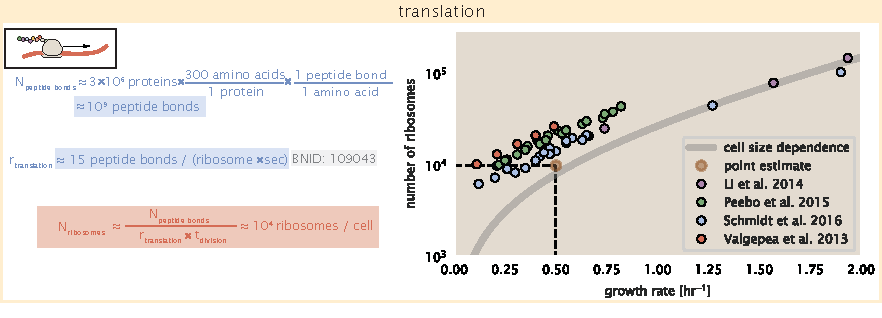
\includegraphics{main_figs/protein_synthesis_main.pdf}
    }
        \caption{\textbf{Estimation of the required number of ribosomes.} Estimation of the
        number of ribosomes required to synthesize 10$^9$ peptide bonds with an
        elongation rate of 15 peptide bonds per second. The
        average abundance of ribosomes is plotted as a function of growth rate.
        Our estimated values are shown for a growth rate of 0.5 hr$^{-1}$.
        Grey lines correspond to the estimated complex abundance calculated at
        different growth rates.} \label{fig:protein_synthesis}

        \figsupp[Estimate and observed abundance and growth rate dependence
        of tRNA ligases.]{Estimation for the number of tRNA synthetases that
        will supply the required amino acid demand. The sum of all tRNA
        synthetases copy numbers are plotted as a function of growth rate
        ([ArgS], [CysS], [GlnS], [GltX], [IleS], [LeuS], [ValS], [AlaS]$_2$,
        [AsnS]$_2$, [AspS]$_2$, [TyrS]$_2$, [TrpS]$_2$, [ThrS]$_2$,
        [SerS]$_2$, [ProS]$_2$, [PheS]$_2$[PheT]$_2$, [MetG]$_2$,
        [lysS]$_2$, [HisS]$_2$, [GlyS]$_2$[GlyQ]$_2$).}{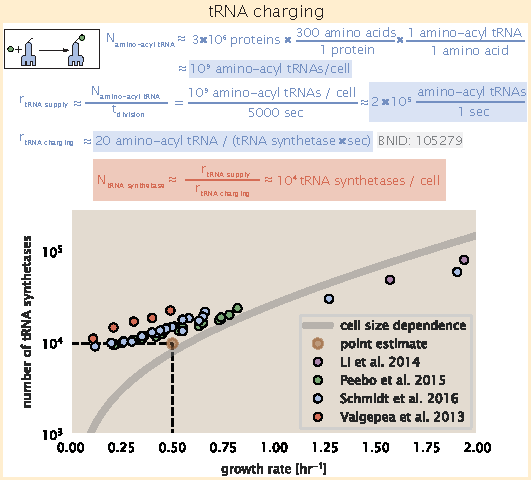
\includegraphics{main_figs/tRNA.pdf}}\label{figsupp:tRNA}
\end{figure}
